\documentclass[1p]{elsarticle_modified}
%\bibliographystyle{elsarticle-num}

%\usepackage[colorlinks]{hyperref}
%\usepackage{abbrmath_seonhwa} %\Abb, \Ascr, \Acal ,\Abf, \Afrak
\usepackage{amsfonts}
\usepackage{amssymb}
\usepackage{amsmath}
\usepackage{amsthm}
\usepackage{scalefnt}
\usepackage{amsbsy}
\usepackage{kotex}
\usepackage{caption}
\usepackage{subfig}
\usepackage{color}
\usepackage{graphicx}
\usepackage{xcolor} %% white, black, red, green, blue, cyan, magenta, yellow
\usepackage{float}
\usepackage{setspace}
\usepackage{hyperref}

\usepackage{tikz}
\usetikzlibrary{arrows}

\usepackage{multirow}
\usepackage{array} % fixed length table
\usepackage{hhline}

%%%%%%%%%%%%%%%%%%%%%
\makeatletter
\renewcommand*\env@matrix[1][\arraystretch]{%
	\edef\arraystretch{#1}%
	\hskip -\arraycolsep
	\let\@ifnextchar\new@ifnextchar
	\array{*\c@MaxMatrixCols c}}
\makeatother %https://tex.stackexchange.com/questions/14071/how-can-i-increase-the-line-spacing-in-a-matrix
%%%%%%%%%%%%%%%

\usepackage[normalem]{ulem}

\newcommand{\msout}[1]{\ifmmode\text{\sout{\ensuremath{#1}}}\else\sout{#1}\fi}
%SOURCE: \msout is \stkout macro in https://tex.stackexchange.com/questions/20609/strikeout-in-math-mode

\newcommand{\cancel}[1]{
	\ifmmode
	{\color{red}\msout{#1}}
	\else
	{\color{red}\sout{#1}}
	\fi
}

\newcommand{\add}[1]{
	{\color{blue}\uwave{#1}}
}

\newcommand{\replace}[2]{
	\ifmmode
	{\color{red}\msout{#1}}{\color{blue}\uwave{#2}}
	\else
	{\color{red}\sout{#1}}{\color{blue}\uwave{#2}}
	\fi
}

\newcommand{\Sol}{\mathcal{S}} %segment
\newcommand{\D}{D} %diagram
\newcommand{\A}{\mathcal{A}} %arc


%%%%%%%%%%%%%%%%%%%%%%%%%%%%%5 test

\def\sl{\operatorname{\textup{SL}}(2,\Cbb)}
\def\psl{\operatorname{\textup{PSL}}(2,\Cbb)}
\def\quan{\mkern 1mu \triangleright \mkern 1mu}

\theoremstyle{definition}
\newtheorem{thm}{Theorem}[section]
\newtheorem{prop}[thm]{Proposition}
\newtheorem{lem}[thm]{Lemma}
\newtheorem{ques}[thm]{Question}
\newtheorem{cor}[thm]{Corollary}
\newtheorem{defn}[thm]{Definition}
\newtheorem{exam}[thm]{Example}
\newtheorem{rmk}[thm]{Remark}
\newtheorem{alg}[thm]{Algorithm}

\newcommand{\I}{\sqrt{-1}}
\begin{document}

%\begin{frontmatter}
%
%\title{Boundary parabolic representations of knots up to 8 crossings}
%
%%% Group authors per affiliation:
%\author{Yunhi Cho} 
%\address{Department of Mathematics, University of Seoul, Seoul, Korea}
%\ead{yhcho@uos.ac.kr}
%
%
%\author{Seonhwa Kim} %\fnref{s_kim}}
%\address{Center for Geometry and Physics, Institute for Basic Science, Pohang, 37673, Korea}
%\ead{ryeona17@ibs.re.kr}
%
%\author{Hyuk Kim}
%\address{Department of Mathematical Sciences, Seoul National University, Seoul 08826, Korea}
%\ead{hyukkim@snu.ac.kr}
%
%\author{Seokbeom Yoon}
%\address{Department of Mathematical Sciences, Seoul National University, Seoul, 08826,  Korea}
%\ead{sbyoon15@snu.ac.kr}
%
%\begin{abstract}
%We find all boundary parabolic representation of knots up to 8 crossings.
%
%\end{abstract}
%\begin{keyword}
%    \MSC[2010] 57M25 
%\end{keyword}
%
%\end{frontmatter}

%\linenumbers
%\tableofcontents
%
\newcommand\colored[1]{\textcolor{white}{\rule[-0.35ex]{0.8em}{1.4ex}}\kern-0.8em\color{red} #1}%
%\newcommand\colored[1]{\textcolor{white}{ #1}\kern-2.17ex	\textcolor{white}{ #1}\kern-1.81ex	\textcolor{white}{ #1}\kern-2.15ex\color{red}#1	}

{\Large $\underline{11a_{296}~(K11a_{296})}$}

\setlength{\tabcolsep}{10pt}
\renewcommand{\arraystretch}{1.6}
\vspace{1cm}\begin{tabular}{m{100pt}>{\centering\arraybackslash}m{274pt}}
\multirow{5}{120pt}{
	\centering
	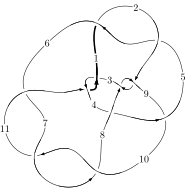
\includegraphics[width=112pt]{../../../GIT/diagram.site/Diagrams/png/545_11a_296.png}\\
\ \ \ A knot diagram\footnotemark}&
\allowdisplaybreaks
\textbf{Linearized knot diagam} \\
\cline{2-2}
 &
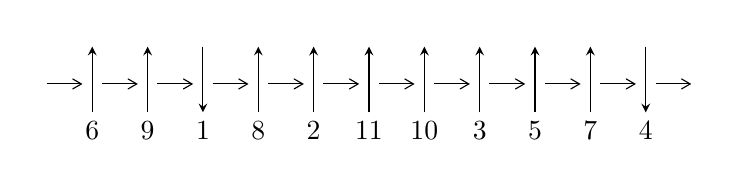
\begin{tikzpicture}[x=20pt, y=17pt]
	% nodes
	\node (C0) at (0, 0) {};
	\node (C1) at (1, 0) {};
	\node (C1U) at (1, +1) {};
	\node (C1D) at (1, -1) {6};

	\node (C2) at (2, 0) {};
	\node (C2U) at (2, +1) {};
	\node (C2D) at (2, -1) {9};

	\node (C3) at (3, 0) {};
	\node (C3U) at (3, +1) {};
	\node (C3D) at (3, -1) {1};

	\node (C4) at (4, 0) {};
	\node (C4U) at (4, +1) {};
	\node (C4D) at (4, -1) {8};

	\node (C5) at (5, 0) {};
	\node (C5U) at (5, +1) {};
	\node (C5D) at (5, -1) {2};

	\node (C6) at (6, 0) {};
	\node (C6U) at (6, +1) {};
	\node (C6D) at (6, -1) {11};

	\node (C7) at (7, 0) {};
	\node (C7U) at (7, +1) {};
	\node (C7D) at (7, -1) {10};

	\node (C8) at (8, 0) {};
	\node (C8U) at (8, +1) {};
	\node (C8D) at (8, -1) {3};

	\node (C9) at (9, 0) {};
	\node (C9U) at (9, +1) {};
	\node (C9D) at (9, -1) {5};

	\node (C10) at (10, 0) {};
	\node (C10U) at (10, +1) {};
	\node (C10D) at (10, -1) {7};

	\node (C11) at (11, 0) {};
	\node (C11U) at (11, +1) {};
	\node (C11D) at (11, -1) {4};
	\node (C12) at (12, 0) {};

	% arrows
	\draw[->,>={angle 60}]
	(C0) edge (C1) (C1) edge (C2) (C2) edge (C3) (C3) edge (C4) (C4) edge (C5) (C5) edge (C6) (C6) edge (C7) (C7) edge (C8) (C8) edge (C9) (C9) edge (C10) (C10) edge (C11) (C11) edge (C12) ;	\draw[->,>=stealth]
	(C1D) edge (C1U) (C2D) edge (C2U) (C3U) edge (C3D) (C4D) edge (C4U) (C5D) edge (C5U) (C6D) edge (C6U) (C7D) edge (C7U) (C8D) edge (C8U) (C9D) edge (C9U) (C10D) edge (C10U) (C11U) edge (C11D) ;
	\end{tikzpicture} \\
\hhline{~~} \\& 
\textbf{Solving Sequence} \\ \cline{2-2} 
 &
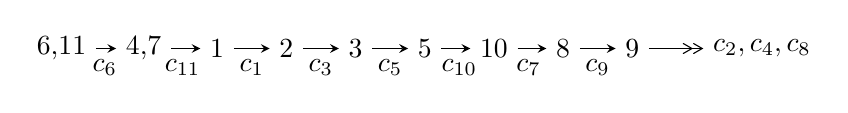
\begin{tikzpicture}[x=25pt, y=7pt]
	% node
	\node (A0) at (-1/8, 0) {6,11};
	\node (A1) at (17/16, 0) {4,7};
	\node (A2) at (17/8, 0) {1};
	\node (A3) at (25/8, 0) {2};
	\node (A4) at (33/8, 0) {3};
	\node (A5) at (41/8, 0) {5};
	\node (A6) at (49/8, 0) {10};
	\node (A7) at (57/8, 0) {8};
	\node (A8) at (65/8, 0) {9};
	\node (C1) at (1/2, -1) {$c_{6}$};
	\node (C2) at (13/8, -1) {$c_{11}$};
	\node (C3) at (21/8, -1) {$c_{1}$};
	\node (C4) at (29/8, -1) {$c_{3}$};
	\node (C5) at (37/8, -1) {$c_{5}$};
	\node (C6) at (45/8, -1) {$c_{10}$};
	\node (C7) at (53/8, -1) {$c_{7}$};
	\node (C8) at (61/8, -1) {$c_{9}$};
	\node (A9) at (10, 0) {$c_{2},c_{4},c_{8}$};

	% edge
	\draw[->,>=stealth]	
	(A0) edge (A1) (A1) edge (A2) (A2) edge (A3) (A3) edge (A4) (A4) edge (A5) (A5) edge (A6) (A6) edge (A7) (A7) edge (A8) ;
	\draw[->>,>={angle 60}]	
	(A8) edge (A9);
\end{tikzpicture} \\ 

\end{tabular} \\

\footnotetext{
The image of knot diagram is generated by the software ``\textbf{Draw programme}" developed by Andrew Bartholomew(\url{http://www.layer8.co.uk/maths/draw/index.htm\#Running-draw}), where we modified some parts for our purpose(\url{https://github.com/CATsTAILs/LinksPainter}).
}\phantom \\ \newline 
\centering \textbf{Ideals for irreducible components\footnotemark of $X_{\text{par}}$} 
 
\begin{align*}
I^u_{1}&=\langle 
-9.00774\times10^{87} u^{70}-2.18808\times10^{87} u^{69}+\cdots+5.70348\times10^{89} b-5.05378\times10^{89},\\
\phantom{I^u_{1}}&\phantom{= \langle  }-5.09051\times10^{89} u^{70}+1.23106\times10^{90} u^{69}+\cdots+5.70348\times10^{89} a-1.93831\times10^{90},\;u^{71}-3 u^{70}+\cdots-6 u+1\rangle \\
I^u_{2}&=\langle 
u^{14}+2 u^{13}+\cdots+b+2,\\
\phantom{I^u_{2}}&\phantom{= \langle  }- u^{15}-7 u^{13}+2 u^{12}-17 u^{11}+15 u^{10}-14 u^9+41 u^8+5 u^7+50 u^6+11 u^5+25 u^4+u^3+4 u^2+a-2 u+1,\\
\phantom{I^u_{2}}&\phantom{= \langle  }u^{16}+2 u^{15}+\cdots+2 u+1\rangle \\
\\
\end{align*}
\raggedright * 2 irreducible components of $\dim_{\mathbb{C}}=0$, with total 87 representations.\\
\footnotetext{All coefficients of polynomials are rational numbers. But the coefficients are sometimes approximated in decimal forms when there is not enough margin.}
\newpage
\renewcommand{\arraystretch}{1}
\centering \section*{I. $I^u_{1}= \langle -9.01\times10^{87} u^{70}-2.19\times10^{87} u^{69}+\cdots+5.70\times10^{89} b-5.05\times10^{89},\;-5.09\times10^{89} u^{70}+1.23\times10^{90} u^{69}+\cdots+5.70\times10^{89} a-1.94\times10^{90},\;u^{71}-3 u^{70}+\cdots-6 u+1 \rangle$}
\flushleft \textbf{(i) Arc colorings}\\
\begin{tabular}{m{7pt} m{180pt} m{7pt} m{180pt} }
\flushright $a_{6}=$&$\begin{pmatrix}1\\0\end{pmatrix}$ \\
\flushright $a_{11}=$&$\begin{pmatrix}0\\u\end{pmatrix}$ \\
\flushright $a_{4}=$&$\begin{pmatrix}0.892526 u^{70}-2.15844 u^{69}+\cdots-10.7951 u+3.39847\\0.0157934 u^{70}+0.00383640 u^{69}+\cdots-7.17845 u+0.886087\end{pmatrix}$ \\
\flushright $a_{7}=$&$\begin{pmatrix}1\\- u^2\end{pmatrix}$ \\
\flushright $a_{1}=$&$\begin{pmatrix}-2.67227 u^{70}+7.45363 u^{69}+\cdots-50.3252 u+5.65629\\0.673792 u^{70}-2.84206 u^{69}+\cdots+8.69069 u-1.27093\end{pmatrix}$ \\
\flushright $a_{2}=$&$\begin{pmatrix}-1.99848 u^{70}+4.61158 u^{69}+\cdots-41.6345 u+4.38536\\0.673792 u^{70}-2.84206 u^{69}+\cdots+8.69069 u-1.27093\end{pmatrix}$ \\
\flushright $a_{3}=$&$\begin{pmatrix}0.937724 u^{70}-2.44311 u^{69}+\cdots+25.2488 u-4.87921\\-0.334153 u^{70}+1.04108 u^{69}+\cdots-5.67570 u+1.49367\end{pmatrix}$ \\
\flushright $a_{5}=$&$\begin{pmatrix}1.09394 u^{70}-2.86528 u^{69}+\cdots-13.4038 u+3.36574\\0.147468 u^{70}-0.313880 u^{69}+\cdots-6.79147 u+0.840422\end{pmatrix}$ \\
\flushright $a_{10}=$&$\begin{pmatrix}- u\\u^3+u\end{pmatrix}$ \\
\flushright $a_{8}=$&$\begin{pmatrix}u^2+1\\- u^4-2 u^2\end{pmatrix}$ \\
\flushright $a_{9}=$&$\begin{pmatrix}-1.33394 u^{70}+4.17244 u^{69}+\cdots-28.8076 u+3.70746\\-0.113697 u^{70}+0.700148 u^{69}+\cdots+8.94630 u-0.936023\end{pmatrix}$\\ \flushright $a_{9}=$&$\begin{pmatrix}-1.33394 u^{70}+4.17244 u^{69}+\cdots-28.8076 u+3.70746\\-0.113697 u^{70}+0.700148 u^{69}+\cdots+8.94630 u-0.936023\end{pmatrix}$\\&\end{tabular}
\flushleft \textbf{(ii) Obstruction class $= -1$}\\~\\
\flushleft \textbf{(iii) Cusp Shapes $= -0.389233 u^{70}+2.15935 u^{69}+\cdots-15.8626 u+7.58410$}\\~\\
\newpage\renewcommand{\arraystretch}{1}
\flushleft \textbf{(iv) u-Polynomials at the component}\newline \\
\begin{tabular}{m{50pt}|m{274pt}}
Crossings & \hspace{64pt}u-Polynomials at each crossing \\
\hline $$\begin{aligned}c_{1},c_{5}\end{aligned}$$&$\begin{aligned}
&u^{71}- u^{70}+\cdots-1361 u-281
\end{aligned}$\\
\hline $$\begin{aligned}c_{2},c_{8}\end{aligned}$$&$\begin{aligned}
&u^{71}+u^{70}+\cdots+117 u-76
\end{aligned}$\\
\hline $$\begin{aligned}c_{3},c_{11}\end{aligned}$$&$\begin{aligned}
&u^{71}-4 u^{70}+\cdots-6 u-13
\end{aligned}$\\
\hline $$\begin{aligned}c_{4}\end{aligned}$$&$\begin{aligned}
&u^{71}-5 u^{70}+\cdots-8378 u-1711
\end{aligned}$\\
\hline $$\begin{aligned}c_{6},c_{7},c_{10}\end{aligned}$$&$\begin{aligned}
&u^{71}+3 u^{70}+\cdots-6 u-1
\end{aligned}$\\
\hline $$\begin{aligned}c_{9}\end{aligned}$$&$\begin{aligned}
&u^{71}+18 u^{69}+\cdots-57052 u-26357
\end{aligned}$\\
\hline
\end{tabular}\\~\\
\newpage\renewcommand{\arraystretch}{1}
\flushleft \textbf{(v) Riley Polynomials at the component}\newline \\
\begin{tabular}{m{50pt}|m{274pt}}
Crossings & \hspace{64pt}Riley Polynomials at each crossing \\
\hline $$\begin{aligned}c_{1},c_{5}\end{aligned}$$&$\begin{aligned}
&y^{71}+59 y^{70}+\cdots-1212265 y-78961
\end{aligned}$\\
\hline $$\begin{aligned}c_{2},c_{8}\end{aligned}$$&$\begin{aligned}
&y^{71}+49 y^{70}+\cdots-79487 y-5776
\end{aligned}$\\
\hline $$\begin{aligned}c_{3},c_{11}\end{aligned}$$&$\begin{aligned}
&y^{71}+36 y^{70}+\cdots+3572 y-169
\end{aligned}$\\
\hline $$\begin{aligned}c_{4}\end{aligned}$$&$\begin{aligned}
&y^{71}+19 y^{70}+\cdots-36750038 y-2927521
\end{aligned}$\\
\hline $$\begin{aligned}c_{6},c_{7},c_{10}\end{aligned}$$&$\begin{aligned}
&y^{71}+73 y^{70}+\cdots-40 y-1
\end{aligned}$\\
\hline $$\begin{aligned}c_{9}\end{aligned}$$&$\begin{aligned}
&y^{71}+36 y^{70}+\cdots-14918431652 y-694691449
\end{aligned}$\\
\hline
\end{tabular}\\~\\
\newpage\flushleft \textbf{(vi) Complex Volumes and Cusp Shapes}
$$\begin{array}{c|c|c}  
\text{Solutions to }I^u_{1}& \I (\text{vol} + \sqrt{-1}CS) & \text{Cusp shape}\\
 \hline 
\begin{aligned}
u &= \phantom{-}0.876704 + 0.516917 I \\
a &= \phantom{-}0.018044 + 1.313340 I \\
b &= \phantom{-}0.76980 - 1.61963 I\end{aligned}
 & -4.30422 + 11.39740 I & \phantom{-0.000000 } 0 \\ \hline\begin{aligned}
u &= \phantom{-}0.876704 - 0.516917 I \\
a &= \phantom{-}0.018044 - 1.313340 I \\
b &= \phantom{-}0.76980 + 1.61963 I\end{aligned}
 & -4.30422 - 11.39740 I & \phantom{-0.000000 } 0 \\ \hline\begin{aligned}
u &= -0.383449 + 0.883215 I \\
a &= \phantom{-}1.004320 - 0.563786 I \\
b &= \phantom{-}0.979718 + 0.596029 I\end{aligned}
 & \phantom{-}1.53313 - 2.60659 I & \phantom{-0.000000 } 0 \\ \hline\begin{aligned}
u &= -0.383449 - 0.883215 I \\
a &= \phantom{-}1.004320 + 0.563786 I \\
b &= \phantom{-}0.979718 - 0.596029 I\end{aligned}
 & \phantom{-}1.53313 + 2.60659 I & \phantom{-0.000000 } 0 \\ \hline\begin{aligned}
u &= -0.952818 + 0.469187 I \\
a &= -0.006177 - 1.082100 I \\
b &= \phantom{-}0.81454 + 1.61178 I\end{aligned}
 & \phantom{-}0.03727 - 4.92803 I & \phantom{-0.000000 } 0 \\ \hline\begin{aligned}
u &= -0.952818 - 0.469187 I \\
a &= -0.006177 + 1.082100 I \\
b &= \phantom{-}0.81454 - 1.61178 I\end{aligned}
 & \phantom{-}0.03727 + 4.92803 I & \phantom{-0.000000 } 0 \\ \hline\begin{aligned}
u &= -0.276228 + 0.874801 I \\
a &= \phantom{-}1.209770 + 0.164013 I \\
b &= -0.335540 + 0.242745 I\end{aligned}
 & -3.52903 - 0.05215 I & \phantom{-0.000000 } 0 \\ \hline\begin{aligned}
u &= -0.276228 - 0.874801 I \\
a &= \phantom{-}1.209770 - 0.164013 I \\
b &= -0.335540 - 0.242745 I\end{aligned}
 & -3.52903 + 0.05215 I & \phantom{-0.000000 } 0 \\ \hline\begin{aligned}
u &= \phantom{-}0.850893 + 0.705002 I \\
a &= -0.934029 - 0.345819 I \\
b &= \phantom{-}0.051753 + 1.245970 I\end{aligned}
 & -4.79765 - 5.63917 I & \phantom{-0.000000 } 0 \\ \hline\begin{aligned}
u &= \phantom{-}0.850893 - 0.705002 I \\
a &= -0.934029 + 0.345819 I \\
b &= \phantom{-}0.051753 - 1.245970 I\end{aligned}
 & -4.79765 + 5.63917 I & \phantom{-0.000000 } 0\\
 \hline 
 \end{array}$$\newpage$$\begin{array}{c|c|c}  
\text{Solutions to }I^u_{1}& \I (\text{vol} + \sqrt{-1}CS) & \text{Cusp shape}\\
 \hline 
\begin{aligned}
u &= \phantom{-}0.805118 + 0.297549 I \\
a &= -0.302889 + 0.998924 I \\
b &= \phantom{-}0.85415 - 1.55688 I\end{aligned}
 & -5.56347 - 1.22600 I & \phantom{-0.000000 } 0 \\ \hline\begin{aligned}
u &= \phantom{-}0.805118 - 0.297549 I \\
a &= -0.302889 - 0.998924 I \\
b &= \phantom{-}0.85415 + 1.55688 I\end{aligned}
 & -5.56347 + 1.22600 I & \phantom{-0.000000 } 0 \\ \hline\begin{aligned}
u &= \phantom{-}0.166244 + 1.177330 I \\
a &= \phantom{-}1.040880 + 0.200780 I \\
b &= \phantom{-}0.133932 - 0.567605 I\end{aligned}
 & -2.99865 + 0.00829 I & \phantom{-0.000000 } 0 \\ \hline\begin{aligned}
u &= \phantom{-}0.166244 - 1.177330 I \\
a &= \phantom{-}1.040880 - 0.200780 I \\
b &= \phantom{-}0.133932 + 0.567605 I\end{aligned}
 & -2.99865 - 0.00829 I & \phantom{-0.000000 } 0 \\ \hline\begin{aligned}
u &= \phantom{-}0.555602 + 0.566754 I \\
a &= -1.208260 + 0.562334 I \\
b &= \phantom{-}0.064611 + 0.675670 I\end{aligned}
 & -6.67179 + 5.48975 I & \phantom{-}1.10039 - 5.62534 I \\ \hline\begin{aligned}
u &= \phantom{-}0.555602 - 0.566754 I \\
a &= -1.208260 - 0.562334 I \\
b &= \phantom{-}0.064611 - 0.675670 I\end{aligned}
 & -6.67179 - 5.48975 I & \phantom{-}1.10039 + 5.62534 I \\ \hline\begin{aligned}
u &= -0.708755 + 0.346572 I \\
a &= -0.357040 + 1.214250 I \\
b &= \phantom{-}0.113056 - 1.348490 I\end{aligned}
 & \phantom{-}3.03135 - 1.49469 I & \phantom{-}12.21917 + 1.87835 I \\ \hline\begin{aligned}
u &= -0.708755 - 0.346572 I \\
a &= -0.357040 - 1.214250 I \\
b &= \phantom{-}0.113056 + 1.348490 I\end{aligned}
 & \phantom{-}3.03135 + 1.49469 I & \phantom{-}12.21917 - 1.87835 I \\ \hline\begin{aligned}
u &= -0.742406 + 0.959669 I \\
a &= -0.626210 + 0.097246 I \\
b &= -0.305996 - 1.152800 I\end{aligned}
 & -1.34036 - 1.05400 I & \phantom{-0.000000 } 0 \\ \hline\begin{aligned}
u &= -0.742406 - 0.959669 I \\
a &= -0.626210 - 0.097246 I \\
b &= -0.305996 + 1.152800 I\end{aligned}
 & -1.34036 + 1.05400 I & \phantom{-0.000000 } 0\\
 \hline 
 \end{array}$$\newpage$$\begin{array}{c|c|c}  
\text{Solutions to }I^u_{1}& \I (\text{vol} + \sqrt{-1}CS) & \text{Cusp shape}\\
 \hline 
\begin{aligned}
u &= -0.190903 + 0.733880 I \\
a &= \phantom{-}0.025776 - 0.589218 I \\
b &= -0.365991 - 0.359203 I\end{aligned}
 & -1.89003 - 1.47574 I & \phantom{-}1.69844 + 5.10987 I \\ \hline\begin{aligned}
u &= -0.190903 - 0.733880 I \\
a &= \phantom{-}0.025776 + 0.589218 I \\
b &= -0.365991 + 0.359203 I\end{aligned}
 & -1.89003 + 1.47574 I & \phantom{-}1.69844 - 5.10987 I \\ \hline\begin{aligned}
u &= \phantom{-}0.569734 + 0.484141 I \\
a &= -0.61345 - 1.53356 I \\
b &= -0.04604 + 1.49792 I\end{aligned}
 & \phantom{-}0.82584 + 5.58849 I & \phantom{-}6.71893 - 8.23388 I \\ \hline\begin{aligned}
u &= \phantom{-}0.569734 - 0.484141 I \\
a &= -0.61345 + 1.53356 I \\
b &= -0.04604 - 1.49792 I\end{aligned}
 & \phantom{-}0.82584 - 5.58849 I & \phantom{-}6.71893 + 8.23388 I \\ \hline\begin{aligned}
u &= -0.653667 + 0.146302 I \\
a &= \phantom{-}0.87774 + 1.79876 I \\
b &= -0.379281 - 1.055800 I\end{aligned}
 & -1.15932 - 3.38797 I & \phantom{-}5.90325 + 4.76662 I \\ \hline\begin{aligned}
u &= -0.653667 - 0.146302 I \\
a &= \phantom{-}0.87774 - 1.79876 I \\
b &= -0.379281 + 1.055800 I\end{aligned}
 & -1.15932 + 3.38797 I & \phantom{-}5.90325 - 4.76662 I \\ \hline\begin{aligned}
u &= \phantom{-}0.000769 + 1.346270 I \\
a &= \phantom{-}0.592643 + 0.337447 I \\
b &= \phantom{-}0.339498 - 1.090940 I\end{aligned}
 & -3.15202 - 1.08459 I & \phantom{-0.000000 } 0 \\ \hline\begin{aligned}
u &= \phantom{-}0.000769 - 1.346270 I \\
a &= \phantom{-}0.592643 - 0.337447 I \\
b &= \phantom{-}0.339498 + 1.090940 I\end{aligned}
 & -3.15202 + 1.08459 I & \phantom{-0.000000 } 0 \\ \hline\begin{aligned}
u &= -0.212829 + 1.337500 I \\
a &= -0.545515 + 0.939906 I \\
b &= -0.73928 - 1.47728 I\end{aligned}
 & -5.79082 - 6.48362 I & \phantom{-0.000000 } 0 \\ \hline\begin{aligned}
u &= -0.212829 - 1.337500 I \\
a &= -0.545515 - 0.939906 I \\
b &= -0.73928 + 1.47728 I\end{aligned}
 & -5.79082 + 6.48362 I & \phantom{-0.000000 } 0\\
 \hline 
 \end{array}$$\newpage$$\begin{array}{c|c|c}  
\text{Solutions to }I^u_{1}& \I (\text{vol} + \sqrt{-1}CS) & \text{Cusp shape}\\
 \hline 
\begin{aligned}
u &= \phantom{-}0.096488 + 1.359540 I \\
a &= \phantom{-}0.246854 - 0.294342 I \\
b &= -0.34390 + 1.89289 I\end{aligned}
 & -8.06307 + 3.83737 I & \phantom{-0.000000 } 0 \\ \hline\begin{aligned}
u &= \phantom{-}0.096488 - 1.359540 I \\
a &= \phantom{-}0.246854 + 0.294342 I \\
b &= -0.34390 - 1.89289 I\end{aligned}
 & -8.06307 - 3.83737 I & \phantom{-0.000000 } 0 \\ \hline\begin{aligned}
u &= \phantom{-}0.177258 + 1.357570 I \\
a &= -0.009719 - 0.403632 I \\
b &= -0.83501 + 1.55183 I\end{aligned}
 & -8.10631 + 3.87908 I & \phantom{-0.000000 } 0 \\ \hline\begin{aligned}
u &= \phantom{-}0.177258 - 1.357570 I \\
a &= -0.009719 + 0.403632 I \\
b &= -0.83501 - 1.55183 I\end{aligned}
 & -8.10631 - 3.87908 I & \phantom{-0.000000 } 0 \\ \hline\begin{aligned}
u &= \phantom{-}0.123250 + 1.376920 I \\
a &= -0.810111 - 0.684516 I \\
b &= -0.97380 + 1.34302 I\end{aligned}
 & -4.05458 + 4.15368 I & \phantom{-0.000000 } 0 \\ \hline\begin{aligned}
u &= \phantom{-}0.123250 - 1.376920 I \\
a &= -0.810111 + 0.684516 I \\
b &= -0.97380 - 1.34302 I\end{aligned}
 & -4.05458 - 4.15368 I & \phantom{-0.000000 } 0 \\ \hline\begin{aligned}
u &= \phantom{-}0.018897 + 1.385550 I \\
a &= -1.241690 - 0.236182 I \\
b &= -1.362110 + 0.377613 I\end{aligned}
 & -3.28165 + 2.64244 I & \phantom{-0.000000 } 0 \\ \hline\begin{aligned}
u &= \phantom{-}0.018897 - 1.385550 I \\
a &= -1.241690 + 0.236182 I \\
b &= -1.362110 - 0.377613 I\end{aligned}
 & -3.28165 - 2.64244 I & \phantom{-0.000000 } 0 \\ \hline\begin{aligned}
u &= \phantom{-}0.481402 + 0.355980 I \\
a &= \phantom{-}0.994444 - 0.755690 I \\
b &= -0.273431 + 0.381017 I\end{aligned}
 & -2.67458 + 1.55489 I & \phantom{-}2.82989 - 4.24710 I \\ \hline\begin{aligned}
u &= \phantom{-}0.481402 - 0.355980 I \\
a &= \phantom{-}0.994444 + 0.755690 I \\
b &= -0.273431 - 0.381017 I\end{aligned}
 & -2.67458 - 1.55489 I & \phantom{-}2.82989 + 4.24710 I\\
 \hline 
 \end{array}$$\newpage$$\begin{array}{c|c|c}  
\text{Solutions to }I^u_{1}& \I (\text{vol} + \sqrt{-1}CS) & \text{Cusp shape}\\
 \hline 
\begin{aligned}
u &= -0.06503 + 1.42398 I \\
a &= \phantom{-}0.662560 - 0.647023 I \\
b &= \phantom{-}0.148769 + 0.759204 I\end{aligned}
 & -4.60407 - 3.10250 I & \phantom{-0.000000 } 0 \\ \hline\begin{aligned}
u &= -0.06503 - 1.42398 I \\
a &= \phantom{-}0.662560 + 0.647023 I \\
b &= \phantom{-}0.148769 - 0.759204 I\end{aligned}
 & -4.60407 + 3.10250 I & \phantom{-0.000000 } 0 \\ \hline\begin{aligned}
u &= -0.05232 + 1.45453 I \\
a &= -0.735490 + 0.335267 I \\
b &= -2.09725 - 1.71117 I\end{aligned}
 & -10.25020 - 4.13818 I & \phantom{-0.000000 } 0 \\ \hline\begin{aligned}
u &= -0.05232 - 1.45453 I \\
a &= -0.735490 - 0.335267 I \\
b &= -2.09725 + 1.71117 I\end{aligned}
 & -10.25020 + 4.13818 I & \phantom{-0.000000 } 0 \\ \hline\begin{aligned}
u &= -0.25007 + 1.45878 I \\
a &= -0.547129 + 0.418576 I \\
b &= -0.61317 - 1.54749 I\end{aligned}
 & -2.82172 - 4.95017 I & \phantom{-0.000000 } 0 \\ \hline\begin{aligned}
u &= -0.25007 - 1.45878 I \\
a &= -0.547129 - 0.418576 I \\
b &= -0.61317 + 1.54749 I\end{aligned}
 & -2.82172 + 4.95017 I & \phantom{-0.000000 } 0 \\ \hline\begin{aligned}
u &= \phantom{-}0.34183 + 1.48836 I \\
a &= \phantom{-}0.599521 + 0.532622 I \\
b &= \phantom{-}1.82790 - 1.33312 I\end{aligned}
 & -11.32690 + 3.07672 I & \phantom{-0.000000 } 0 \\ \hline\begin{aligned}
u &= \phantom{-}0.34183 - 1.48836 I \\
a &= \phantom{-}0.599521 - 0.532622 I \\
b &= \phantom{-}1.82790 + 1.33312 I\end{aligned}
 & -11.32690 - 3.07672 I & \phantom{-0.000000 } 0 \\ \hline\begin{aligned}
u &= \phantom{-}0.19479 + 1.51543 I \\
a &= -0.459769 + 0.827837 I \\
b &= \phantom{-}0.114814 - 0.131344 I\end{aligned}
 & -13.4581 + 8.2834 I & \phantom{-0.000000 } 0 \\ \hline\begin{aligned}
u &= \phantom{-}0.19479 - 1.51543 I \\
a &= -0.459769 - 0.827837 I \\
b &= \phantom{-}0.114814 + 0.131344 I\end{aligned}
 & -13.4581 - 8.2834 I & \phantom{-0.000000 } 0\\
 \hline 
 \end{array}$$\newpage$$\begin{array}{c|c|c}  
\text{Solutions to }I^u_{1}& \I (\text{vol} + \sqrt{-1}CS) & \text{Cusp shape}\\
 \hline 
\begin{aligned}
u &= \phantom{-}0.19607 + 1.51746 I \\
a &= -0.670319 - 0.456053 I \\
b &= -0.52830 + 1.86550 I\end{aligned}
 & -5.78366 + 8.41270 I & \phantom{-0.000000 } 0 \\ \hline\begin{aligned}
u &= \phantom{-}0.19607 - 1.51746 I \\
a &= -0.670319 + 0.456053 I \\
b &= -0.52830 - 1.86550 I\end{aligned}
 & -5.78366 - 8.41270 I & \phantom{-0.000000 } 0 \\ \hline\begin{aligned}
u &= -0.14626 + 1.54836 I \\
a &= -0.223801 - 0.693017 I \\
b &= -0.069496 + 0.154353 I\end{aligned}
 & -9.50943 - 3.27093 I & \phantom{-0.000000 } 0 \\ \hline\begin{aligned}
u &= -0.14626 - 1.54836 I \\
a &= -0.223801 + 0.693017 I \\
b &= -0.069496 - 0.154353 I\end{aligned}
 & -9.50943 + 3.27093 I & \phantom{-0.000000 } 0 \\ \hline\begin{aligned}
u &= \phantom{-}0.420094 + 0.080132 I \\
a &= \phantom{-}0.54577 - 2.67604 I \\
b &= -0.403742 + 1.076110 I\end{aligned}
 & \phantom{-}0.66143 + 2.25848 I & \phantom{-}4.43494 + 0.57709 I \\ \hline\begin{aligned}
u &= \phantom{-}0.420094 - 0.080132 I \\
a &= \phantom{-}0.54577 + 2.67604 I \\
b &= -0.403742 - 1.076110 I\end{aligned}
 & \phantom{-}0.66143 - 2.25848 I & \phantom{-}4.43494 - 0.57709 I \\ \hline\begin{aligned}
u &= \phantom{-}0.31389 + 1.54199 I \\
a &= \phantom{-}0.690616 + 0.664349 I \\
b &= \phantom{-}1.38403 - 1.60738 I\end{aligned}
 & -10.9839 + 15.7452 I & \phantom{-0.000000 } 0 \\ \hline\begin{aligned}
u &= \phantom{-}0.31389 - 1.54199 I \\
a &= \phantom{-}0.690616 - 0.664349 I \\
b &= \phantom{-}1.38403 + 1.60738 I\end{aligned}
 & -10.9839 - 15.7452 I & \phantom{-0.000000 } 0 \\ \hline\begin{aligned}
u &= -0.32953 + 1.53939 I \\
a &= \phantom{-}0.683207 - 0.587683 I \\
b &= \phantom{-}1.50202 + 1.41422 I\end{aligned}
 & -6.50526 - 9.54418 I & \phantom{-0.000000 } 0 \\ \hline\begin{aligned}
u &= -0.32953 - 1.53939 I \\
a &= \phantom{-}0.683207 + 0.587683 I \\
b &= \phantom{-}1.50202 - 1.41422 I\end{aligned}
 & -6.50526 + 9.54418 I & \phantom{-0.000000 } 0\\
 \hline 
 \end{array}$$\newpage$$\begin{array}{c|c|c}  
\text{Solutions to }I^u_{1}& \I (\text{vol} + \sqrt{-1}CS) & \text{Cusp shape}\\
 \hline 
\begin{aligned}
u &= \phantom{-}0.350278 + 0.238783 I \\
a &= \phantom{-}2.06396 + 2.08046 I \\
b &= -0.108087 - 0.747622 I\end{aligned}
 & \phantom{-}0.99996 - 2.28586 I & \phantom{-}9.25040 + 1.43697 I \\ \hline\begin{aligned}
u &= \phantom{-}0.350278 - 0.238783 I \\
a &= \phantom{-}2.06396 - 2.08046 I \\
b &= -0.108087 + 0.747622 I\end{aligned}
 & \phantom{-}0.99996 + 2.28586 I & \phantom{-}9.25040 - 1.43697 I \\ \hline\begin{aligned}
u &= -0.380862\phantom{ +0.000000I} \\
a &= \phantom{-}0.547449\phantom{ +0.000000I} \\
b &= \phantom{-}0.250181\phantom{ +0.000000I}\end{aligned}
 & \phantom{-}0.684340\phantom{ +0.000000I} & \phantom{-}14.6690\phantom{ +0.000000I} \\ \hline\begin{aligned}
u &= -0.00681 + 1.62560 I \\
a &= \phantom{-}0.370034 + 0.196828 I \\
b &= -0.791967 - 0.211199 I\end{aligned}
 & -12.04640 - 0.66622 I & \phantom{-0.000000 } 0 \\ \hline\begin{aligned}
u &= -0.00681 - 1.62560 I \\
a &= \phantom{-}0.370034 - 0.196828 I \\
b &= -0.791967 + 0.211199 I\end{aligned}
 & -12.04640 + 0.66622 I & \phantom{-0.000000 } 0 \\ \hline\begin{aligned}
u &= \phantom{-}0.18915 + 1.65621 I \\
a &= -0.370196 + 0.320048 I \\
b &= -0.241587 + 0.177123 I\end{aligned}
 & -12.95250 - 1.69138 I & \phantom{-0.000000 } 0 \\ \hline\begin{aligned}
u &= \phantom{-}0.18915 - 1.65621 I \\
a &= -0.370196 - 0.320048 I \\
b &= -0.241587 - 0.177123 I\end{aligned}
 & -12.95250 + 1.69138 I & \phantom{-0.000000 } 0 \\ \hline\begin{aligned}
u &= \phantom{-}0.033849 + 0.258899 I \\
a &= \phantom{-}4.95781 - 0.70188 I \\
b &= -0.156325 - 0.185251 I\end{aligned}
 & \phantom{-}1.05941 - 2.33356 I & \phantom{-}9.20153 - 2.18443 I \\ \hline\begin{aligned}
u &= \phantom{-}0.033849 - 0.258899 I \\
a &= \phantom{-}4.95781 + 0.70188 I \\
b &= -0.156325 + 0.185251 I\end{aligned}
 & \phantom{-}1.05941 + 2.33356 I & \phantom{-}9.20153 + 2.18443 I \\ \hline\begin{aligned}
u &= -0.100795 + 0.225172 I \\
a &= -2.19587 + 2.54396 I \\
b &= -1.25338 - 1.68214 I\end{aligned}
 & -4.54187 - 3.47725 I & \phantom{-}1.03919 + 11.73810 I\\
 \hline 
 \end{array}$$\newpage$$\begin{array}{c|c|c}  
\text{Solutions to }I^u_{1}& \I (\text{vol} + \sqrt{-1}CS) & \text{Cusp shape}\\
 \hline 
\begin{aligned}
u &= -0.100795 - 0.225172 I \\
a &= -2.19587 - 2.54396 I \\
b &= -1.25338 + 1.68214 I\end{aligned}
 & -4.54187 + 3.47725 I & \phantom{-}1.03919 - 11.73810 I\\
 \hline 
 \end{array}$$\newpage\newpage\renewcommand{\arraystretch}{1}
\centering \section*{II. $I^u_{2}= \langle u^{14}+2 u^{13}+\cdots+b+2,\;- u^{15}-7 u^{13}+\cdots+a+1,\;u^{16}+2 u^{15}+\cdots+2 u+1 \rangle$}
\flushleft \textbf{(i) Arc colorings}\\
\begin{tabular}{m{7pt} m{180pt} m{7pt} m{180pt} }
\flushright $a_{6}=$&$\begin{pmatrix}1\\0\end{pmatrix}$ \\
\flushright $a_{11}=$&$\begin{pmatrix}0\\u\end{pmatrix}$ \\
\flushright $a_{4}=$&$\begin{pmatrix}u^{15}+7 u^{13}+\cdots+2 u-1\\- u^{14}-2 u^{13}+\cdots-4 u-2\end{pmatrix}$ \\
\flushright $a_{7}=$&$\begin{pmatrix}1\\- u^2\end{pmatrix}$ \\
\flushright $a_{1}=$&$\begin{pmatrix}- u^{14}-3 u^{13}+\cdots-3 u-4\\- u^{15}-2 u^{14}+\cdots+2 u^2- u\end{pmatrix}$ \\
\flushright $a_{2}=$&$\begin{pmatrix}- u^{15}-3 u^{14}+\cdots-4 u-4\\- u^{15}-2 u^{14}+\cdots+2 u^2- u\end{pmatrix}$ \\
\flushright $a_{3}=$&$\begin{pmatrix}- u^{15}- u^{14}+\cdots- u-2\\- u^{14}-2 u^{13}+\cdots-4 u-1\end{pmatrix}$ \\
\flushright $a_{5}=$&$\begin{pmatrix}u^{15}+7 u^{13}+\cdots-6 u^2-1\\- u^5- u^4-3 u^3-2 u^2-2 u-1\end{pmatrix}$ \\
\flushright $a_{10}=$&$\begin{pmatrix}- u\\u^3+u\end{pmatrix}$ \\
\flushright $a_{8}=$&$\begin{pmatrix}u^2+1\\- u^4-2 u^2\end{pmatrix}$ \\
\flushright $a_{9}=$&$\begin{pmatrix}-2 u^{15}-4 u^{14}+\cdots- u-1\\- u^{13}-2 u^{12}+\cdots-9 u^3-2 u^2\end{pmatrix}$\\ \flushright $a_{9}=$&$\begin{pmatrix}-2 u^{15}-4 u^{14}+\cdots- u-1\\- u^{13}-2 u^{12}+\cdots-9 u^3-2 u^2\end{pmatrix}$\\&\end{tabular}
\flushleft \textbf{(ii) Obstruction class $= 1$}\\~\\
\flushleft \textbf{(iii) Cusp Shapes $= 8 u^{15}+11 u^{14}+75 u^{13}+88 u^{12}+284 u^{11}+269 u^{10}+546 u^9+386 u^8+544 u^7+244 u^6+249 u^5+41 u^4+44 u^3-2 u^2+14 u+7$}\\~\\
\newpage\renewcommand{\arraystretch}{1}
\flushleft \textbf{(iv) u-Polynomials at the component}\newline \\
\begin{tabular}{m{50pt}|m{274pt}}
Crossings & \hspace{64pt}u-Polynomials at each crossing \\
\hline $$\begin{aligned}c_{1}\end{aligned}$$&$\begin{aligned}
&u^{16}+8 u^{14}+\cdots+3 u+1
\end{aligned}$\\
\hline $$\begin{aligned}c_{2}\end{aligned}$$&$\begin{aligned}
&u^{16}+5 u^{14}+\cdots+4 u^2+1
\end{aligned}$\\
\hline $$\begin{aligned}c_{3}\end{aligned}$$&$\begin{aligned}
&u^{16}+3 u^{15}+\cdots+8 u^2+1
\end{aligned}$\\
\hline $$\begin{aligned}c_{4}\end{aligned}$$&$\begin{aligned}
&u^{16}+u^{13}+\cdots-7 u^2+1
\end{aligned}$\\
\hline $$\begin{aligned}c_{5}\end{aligned}$$&$\begin{aligned}
&u^{16}+8 u^{14}+\cdots-3 u+1
\end{aligned}$\\
\hline $$\begin{aligned}c_{6},c_{7}\end{aligned}$$&$\begin{aligned}
&u^{16}+2 u^{15}+\cdots+2 u+1
\end{aligned}$\\
\hline $$\begin{aligned}c_{8}\end{aligned}$$&$\begin{aligned}
&u^{16}+5 u^{14}+\cdots+4 u^2+1
\end{aligned}$\\
\hline $$\begin{aligned}c_{9}\end{aligned}$$&$\begin{aligned}
&u^{16}+u^{15}+\cdots+6 u^2+1
\end{aligned}$\\
\hline $$\begin{aligned}c_{10}\end{aligned}$$&$\begin{aligned}
&u^{16}-2 u^{15}+\cdots-2 u+1
\end{aligned}$\\
\hline $$\begin{aligned}c_{11}\end{aligned}$$&$\begin{aligned}
&u^{16}-3 u^{15}+\cdots+8 u^2+1
\end{aligned}$\\
\hline
\end{tabular}\\~\\
\newpage\renewcommand{\arraystretch}{1}
\flushleft \textbf{(v) Riley Polynomials at the component}\newline \\
\begin{tabular}{m{50pt}|m{274pt}}
Crossings & \hspace{64pt}Riley Polynomials at each crossing \\
\hline $$\begin{aligned}c_{1},c_{5}\end{aligned}$$&$\begin{aligned}
&y^{16}+16 y^{15}+\cdots+13 y+1
\end{aligned}$\\
\hline $$\begin{aligned}c_{2},c_{8}\end{aligned}$$&$\begin{aligned}
&y^{16}+10 y^{15}+\cdots+8 y+1
\end{aligned}$\\
\hline $$\begin{aligned}c_{3},c_{11}\end{aligned}$$&$\begin{aligned}
&y^{16}+13 y^{15}+\cdots+16 y+1
\end{aligned}$\\
\hline $$\begin{aligned}c_{4}\end{aligned}$$&$\begin{aligned}
&y^{16}-2 y^{14}+\cdots-14 y+1
\end{aligned}$\\
\hline $$\begin{aligned}c_{6},c_{7},c_{10}\end{aligned}$$&$\begin{aligned}
&y^{16}+18 y^{15}+\cdots+4 y+1
\end{aligned}$\\
\hline $$\begin{aligned}c_{9}\end{aligned}$$&$\begin{aligned}
&y^{16}+5 y^{15}+\cdots+12 y+1
\end{aligned}$\\
\hline
\end{tabular}\\~\\
\newpage\flushleft \textbf{(vi) Complex Volumes and Cusp Shapes}
$$\begin{array}{c|c|c}  
\text{Solutions to }I^u_{2}& \I (\text{vol} + \sqrt{-1}CS) & \text{Cusp shape}\\
 \hline 
\begin{aligned}
u &= -0.569342 + 1.028560 I \\
a &= \phantom{-}0.720411 - 0.176385 I \\
b &= \phantom{-}0.175330 + 0.986553 I\end{aligned}
 & -0.549860 - 0.999226 I & \phantom{-}9.35133 + 0.51407 I \\ \hline\begin{aligned}
u &= -0.569342 - 1.028560 I \\
a &= \phantom{-}0.720411 + 0.176385 I \\
b &= \phantom{-}0.175330 - 0.986553 I\end{aligned}
 & -0.549860 + 0.999226 I & \phantom{-}9.35133 - 0.51407 I \\ \hline\begin{aligned}
u &= -0.324061 + 0.738568 I \\
a &= -1.22712 + 0.86928 I \\
b &= -1.167210 - 0.652672 I\end{aligned}
 & \phantom{-}0.66827 - 2.96805 I & \phantom{-}2.18241 + 5.99537 I \\ \hline\begin{aligned}
u &= -0.324061 - 0.738568 I \\
a &= -1.22712 - 0.86928 I \\
b &= -1.167210 + 0.652672 I\end{aligned}
 & \phantom{-}0.66827 + 2.96805 I & \phantom{-}2.18241 - 5.99537 I \\ \hline\begin{aligned}
u &= -0.051468 + 1.266120 I \\
a &= \phantom{-}1.278820 + 0.261068 I \\
b &= \phantom{-}0.427098 + 0.016868 I\end{aligned}
 & -2.01678 + 1.79591 I & \phantom{-}6.94894 - 2.52988 I \\ \hline\begin{aligned}
u &= -0.051468 - 1.266120 I \\
a &= \phantom{-}1.278820 - 0.261068 I \\
b &= \phantom{-}0.427098 - 0.016868 I\end{aligned}
 & -2.01678 - 1.79591 I & \phantom{-}6.94894 + 2.52988 I \\ \hline\begin{aligned}
u &= \phantom{-}0.168287 + 1.312890 I \\
a &= -0.500784 - 0.449767 I \\
b &= -1.55170 + 2.17075 I\end{aligned}
 & -7.83940 + 4.87519 I & \phantom{-}1.58436 - 7.54746 I \\ \hline\begin{aligned}
u &= \phantom{-}0.168287 - 1.312890 I \\
a &= -0.500784 + 0.449767 I \\
b &= -1.55170 - 2.17075 I\end{aligned}
 & -7.83940 - 4.87519 I & \phantom{-}1.58436 + 7.54746 I \\ \hline\begin{aligned}
u &= -0.18168 + 1.42029 I \\
a &= -0.619856 + 0.736296 I \\
b &= -0.71287 - 1.31954 I\end{aligned}
 & -4.56313 - 5.40512 I & \phantom{-}2.67129 + 5.45372 I \\ \hline\begin{aligned}
u &= -0.18168 - 1.42029 I \\
a &= -0.619856 - 0.736296 I \\
b &= -0.71287 + 1.31954 I\end{aligned}
 & -4.56313 + 5.40512 I & \phantom{-}2.67129 - 5.45372 I\\
 \hline 
 \end{array}$$\newpage$$\begin{array}{c|c|c}  
\text{Solutions to }I^u_{2}& \I (\text{vol} + \sqrt{-1}CS) & \text{Cusp shape}\\
 \hline 
\begin{aligned}
u &= -0.458536 + 0.295995 I \\
a &= -0.30047 + 2.31517 I \\
b &= -0.443631 - 0.902773 I\end{aligned}
 & \phantom{-}0.92810 - 3.00419 I & \phantom{-}8.30090 + 9.42735 I \\ \hline\begin{aligned}
u &= -0.458536 - 0.295995 I \\
a &= -0.30047 - 2.31517 I \\
b &= -0.443631 + 0.902773 I\end{aligned}
 & \phantom{-}0.92810 + 3.00419 I & \phantom{-}8.30090 - 9.42735 I \\ \hline\begin{aligned}
u &= \phantom{-}0.349990 + 0.344981 I \\
a &= \phantom{-}1.33662 + 0.55629 I \\
b &= -0.74370 - 1.67764 I\end{aligned}
 & -4.41668 - 2.95405 I & \phantom{-}4.95739 - 2.07123 I \\ \hline\begin{aligned}
u &= \phantom{-}0.349990 - 0.344981 I \\
a &= \phantom{-}1.33662 - 0.55629 I \\
b &= -0.74370 + 1.67764 I\end{aligned}
 & -4.41668 + 2.95405 I & \phantom{-}4.95739 + 2.07123 I \\ \hline\begin{aligned}
u &= \phantom{-}0.06681 + 1.63596 I \\
a &= \phantom{-}0.312384 - 0.028797 I \\
b &= -0.483326 - 0.701860 I\end{aligned}
 & -11.81930 - 1.32705 I & \phantom{-}4.00338 + 5.75939 I \\ \hline\begin{aligned}
u &= \phantom{-}0.06681 - 1.63596 I \\
a &= \phantom{-}0.312384 + 0.028797 I \\
b &= -0.483326 + 0.701860 I\end{aligned}
 & -11.81930 + 1.32705 I & \phantom{-}4.00338 - 5.75939 I\\
 \hline 
 \end{array}$$\newpage
\newpage\renewcommand{\arraystretch}{1}
\centering \section*{ III. u-Polynomials}
\begin{tabular}{m{50pt}|m{274pt}}
Crossings & \hspace{64pt}u-Polynomials at each crossing \\
\hline $$\begin{aligned}c_{1}\end{aligned}$$&$\begin{aligned}
&(u^{16}+8 u^{14}+\cdots+3 u+1)(u^{71}- u^{70}+\cdots-1361 u-281)
\end{aligned}$\\
\hline $$\begin{aligned}c_{2}\end{aligned}$$&$\begin{aligned}
&(u^{16}+5 u^{14}+\cdots+4 u^2+1)(u^{71}+u^{70}+\cdots+117 u-76)
\end{aligned}$\\
\hline $$\begin{aligned}c_{3}\end{aligned}$$&$\begin{aligned}
&(u^{16}+3 u^{15}+\cdots+8 u^2+1)(u^{71}-4 u^{70}+\cdots-6 u-13)
\end{aligned}$\\
\hline $$\begin{aligned}c_{4}\end{aligned}$$&$\begin{aligned}
&(u^{16}+u^{13}+\cdots-7 u^2+1)(u^{71}-5 u^{70}+\cdots-8378 u-1711)
\end{aligned}$\\
\hline $$\begin{aligned}c_{5}\end{aligned}$$&$\begin{aligned}
&(u^{16}+8 u^{14}+\cdots-3 u+1)(u^{71}- u^{70}+\cdots-1361 u-281)
\end{aligned}$\\
\hline $$\begin{aligned}c_{6},c_{7}\end{aligned}$$&$\begin{aligned}
&(u^{16}+2 u^{15}+\cdots+2 u+1)(u^{71}+3 u^{70}+\cdots-6 u-1)
\end{aligned}$\\
\hline $$\begin{aligned}c_{8}\end{aligned}$$&$\begin{aligned}
&(u^{16}+5 u^{14}+\cdots+4 u^2+1)(u^{71}+u^{70}+\cdots+117 u-76)
\end{aligned}$\\
\hline $$\begin{aligned}c_{9}\end{aligned}$$&$\begin{aligned}
&(u^{16}+u^{15}+\cdots+6 u^2+1)(u^{71}+18 u^{69}+\cdots-57052 u-26357)
\end{aligned}$\\
\hline $$\begin{aligned}c_{10}\end{aligned}$$&$\begin{aligned}
&(u^{16}-2 u^{15}+\cdots-2 u+1)(u^{71}+3 u^{70}+\cdots-6 u-1)
\end{aligned}$\\
\hline $$\begin{aligned}c_{11}\end{aligned}$$&$\begin{aligned}
&(u^{16}-3 u^{15}+\cdots+8 u^2+1)(u^{71}-4 u^{70}+\cdots-6 u-13)
\end{aligned}$\\
\hline
\end{tabular}\newpage\renewcommand{\arraystretch}{1}
\centering \section*{ IV. Riley Polynomials}
\begin{tabular}{m{50pt}|m{274pt}}
Crossings & \hspace{64pt}Riley Polynomials at each crossing \\
\hline $$\begin{aligned}c_{1},c_{5}\end{aligned}$$&$\begin{aligned}
&(y^{16}+16 y^{15}+\cdots+13 y+1)(y^{71}+59 y^{70}+\cdots-1212265 y-78961)
\end{aligned}$\\
\hline $$\begin{aligned}c_{2},c_{8}\end{aligned}$$&$\begin{aligned}
&(y^{16}+10 y^{15}+\cdots+8 y+1)(y^{71}+49 y^{70}+\cdots-79487 y-5776)
\end{aligned}$\\
\hline $$\begin{aligned}c_{3},c_{11}\end{aligned}$$&$\begin{aligned}
&(y^{16}+13 y^{15}+\cdots+16 y+1)(y^{71}+36 y^{70}+\cdots+3572 y-169)
\end{aligned}$\\
\hline $$\begin{aligned}c_{4}\end{aligned}$$&$\begin{aligned}
&(y^{16}-2 y^{14}+\cdots-14 y+1)\\
&\cdot(y^{71}+19 y^{70}+\cdots-36750038 y-2927521)
\end{aligned}$\\
\hline $$\begin{aligned}c_{6},c_{7},c_{10}\end{aligned}$$&$\begin{aligned}
&(y^{16}+18 y^{15}+\cdots+4 y+1)(y^{71}+73 y^{70}+\cdots-40 y-1)
\end{aligned}$\\
\hline $$\begin{aligned}c_{9}\end{aligned}$$&$\begin{aligned}
&(y^{16}+5 y^{15}+\cdots+12 y+1)\\
&\cdot(y^{71}+36 y^{70}+\cdots-14918431652 y-694691449)
\end{aligned}$\\
\hline
\end{tabular}
\vskip 2pc
\end{document}